\section{Quantum Double Model V}
\subsection{Review - multiple flux excitations and GSD}
Last time, we supposed we had trapped $n$ flux excitations $c_1, \ldots c_n$ at plaquettes $p_1, \ldots p_n$. What we showed last time was - perhaps unexpectedly - the Hamiltonian had multiple degenerate ground states, labelled by ordered $n$-tuples:
\begin{equation}
    \set{(g_1, \ldots, g_n): g_i \in C_i, g_1\ldots g_n=1}
\end{equation}
we found a ground state for each of these $n$-tuples, modulo uniform conjugation:
\begin{equation}
    \ket{g_1, \ldots g_n} = \ket{hg_1h^{-1}, \ldots, hg_nh^{-1}}.
\end{equation}
These are all ground states with trivial total topological charge (which means that we are thinking about ground states that can be created by some local operation).

One point that we want to emphasize from last time - the GSD is slightly special, in the sense that all of the degenerate states are locally indistinguishable. The simplest measurement we could do to distinguish the states involves a string operator that would go around more than one plaquette. Additionally, the size of the degeneracy does not go as a product of the internal degrees of freedom; there is a collective degeneracy coming from defects, here a power of the size of the conjugacy class. This peculiar GSD is the defining characteristic of non-Abelian anyons.

\subsection{Braiding of fluxes}
Let us have $n$ fluxes $c_1, \ldots c_n$ and then exchange $c_1, c_2$ (by some adiabatic evolution). 

\begin{center}
    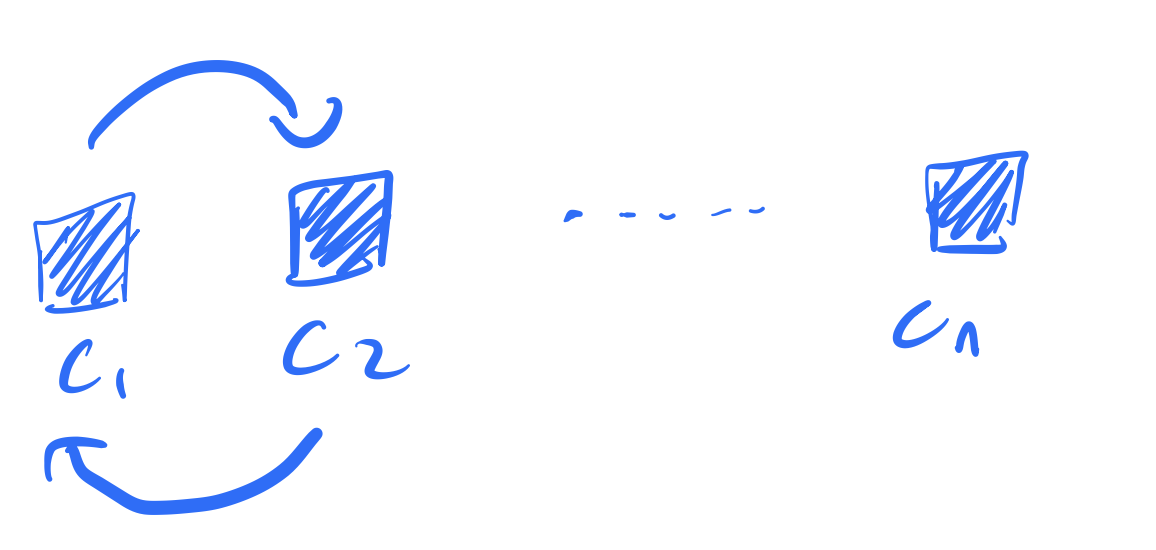
\includegraphics[scale=0.35]{Lectures/Images/lec10-fluxswap.png}
\end{center}

This braiding operation (since we do it adiabatically) leads to another ground state. If the fluxes are of the same type, then we get the same ground state as we started with, if the fluxes are of different types, we will generically have a different ground state. Either way, we end up with the ground state of a new Hamiltonian:
\begin{equation}
    \ket{g_1, g_2, \ldots, g_n} \stackrel{\text{braid}}{\to} \sum_{g_i'}(\text{coeff.})\ket{g_1', g_2', \ldots g_n'}
\end{equation}
Let us compute the RHS, up to a phase. With abelian anyons, we get dynamical phases (separate from the topological Berry phase). Here, we will not worry so much about it because we are dealing with Abelian anyons. So, all the details about, e.g., subtraction schemes we need not concern ourselves with.

Let's recall the definition:
\begin{equation}
    \ket{g_1, \ldots, g_n} = \prod_s A(s)\ket{g_1, \ldots g_n}_0
\end{equation}

Where (focusing on the first two fluxes):

\begin{center}
    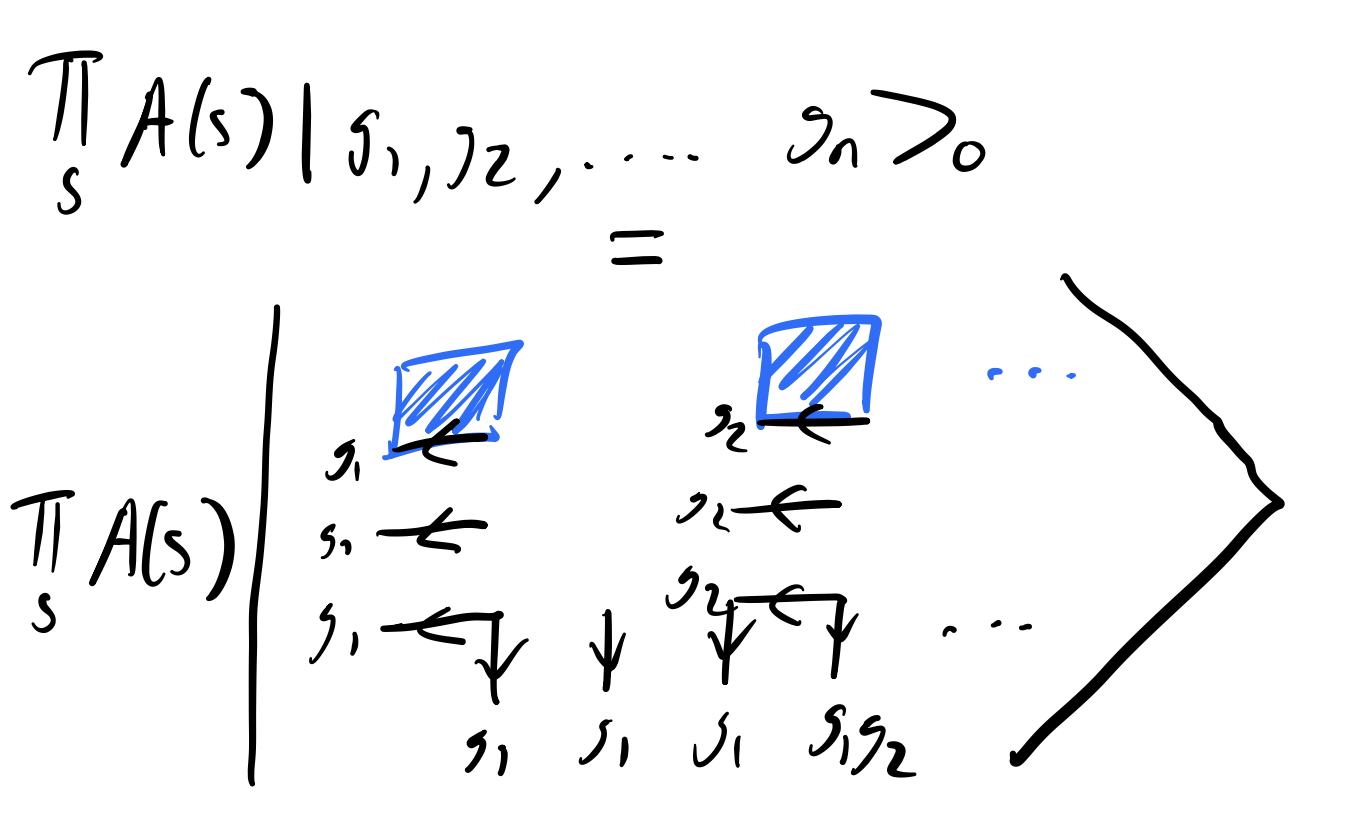
\includegraphics[scale=0.35]{Lectures/Images/lec10-gstate.png}
\end{center}

The final state we can just intuitively write down/guess on the level of the unprojected state, by imagining the operations it would require to move the fluxes in the unprojected setup:

\begin{center}
    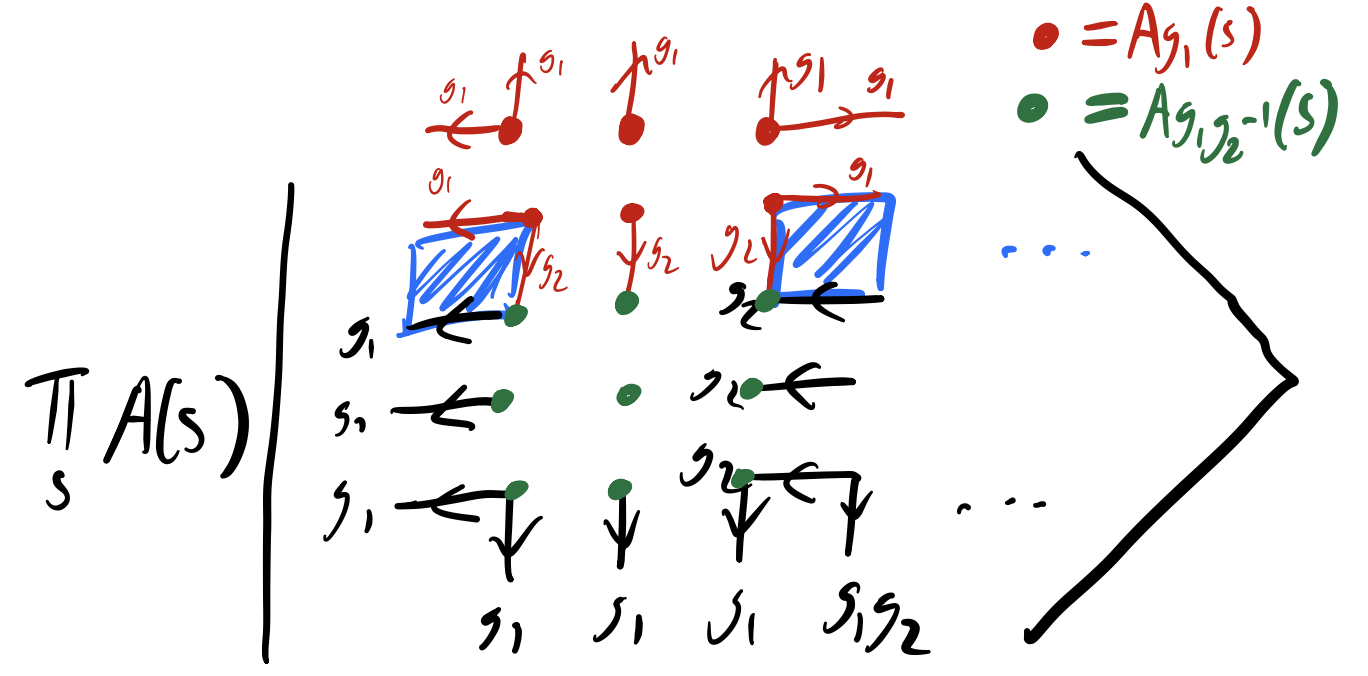
\includegraphics[scale=0.35]{Lectures/Images/lec10-gstategaugeequiv.png}
\end{center}

The second picture is gauge equivalent to the first, up to an $A_{g_1}(s)$ on the red dots and $A_{g_1g_2^{-1}}(s)$ on the green. This gives us:

\begin{center}
    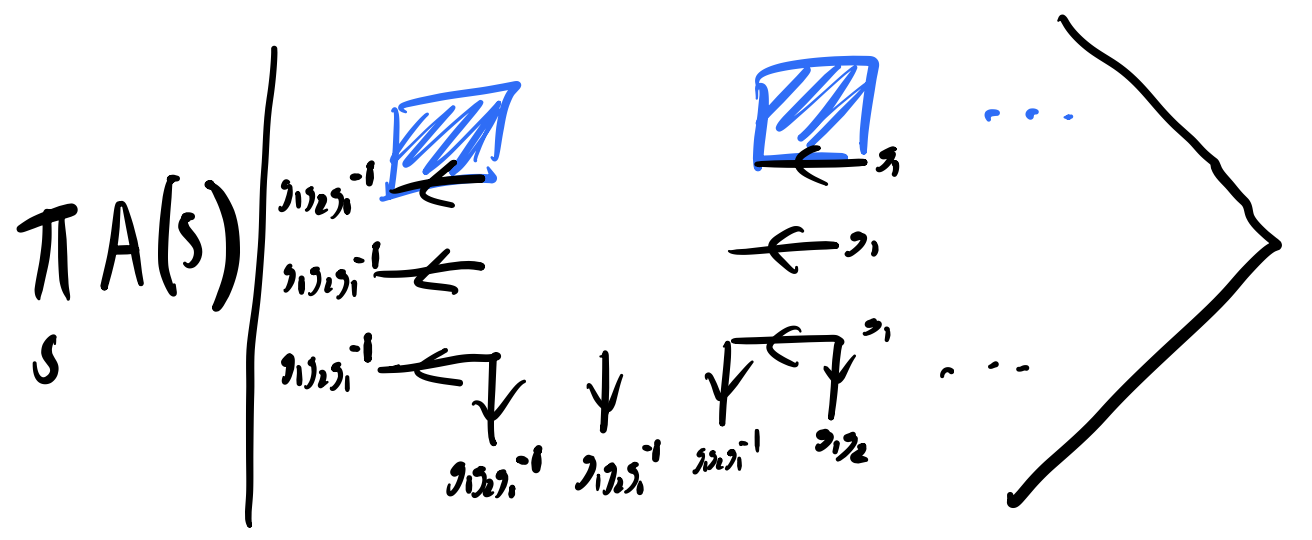
\includegraphics[scale=0.35]{Lectures/Images/lec10-swappedstate.png}
\end{center}

Thus, using our notation for labelling these states, the final result is:
\begin{equation}
    \prod_s A(s)\ket{g_1g_2g_1^{-1}, g_1, \ldots, g_n}_0 = \ket{g_1g_2g_1^{-1}, g_1, \ldots, g_n}.
\end{equation}
Note that in the Abelian case, $g_1g_2g_1^{-1} = g_2$ so we just get the swap of $g_1, g_2$.

More generally, if we exchange fluxes $i, i+1$:
\begin{equation}\label{eq:fluxswaps}
    \boxed{\ket{\ldots, g_i, g_{i+1}, \ldots} \to \ket{\ldots, g_i g_{i+1}g_i^{-1}, g_i, \ldots}}
\end{equation}
which completely defines the braiding of fluxes.

A consistency check; the $g_1\ldots g_n = 1$ condition must be preserved. Indeed, the exchange (which swaps $g_i, g_{i+1}$ and then conjugates $g_{i+1}$) preserves this product.

For simplicity, let us specialize to the case where all the fluxes are the same, $C_1 = C_2 = \ldots = C_n = C$. Now, the Hamiltonian returns to itself, so we can view each braid as defining a $D \times D$ unitary transformation on the set of degenerate of $D$ degenerate ground states (of a fixed Hamiltonian). These define what are known as the \emph{braid matrices}. Eq. \eqref{eq:fluxswaps} gives us an explicit formula for the braid matrices corresponding to clockwise exchanges. Together with their inverses, clockwise exchanges are the generators of the braid group, so this fully defines braiding.

Two properties of (flux) braid matrices:
\begin{enumerate}
    \item Braid matrices are all permutation matrices, in the $\ket{g_1, \ldots, g_n}$ basis. Acting on a particular basis element, we get a single basis element back (as opposed to a linear combination of such basis elements). This is specific to fluxes.
    \item Braid matrices generally do not commute with each other. The outcome is dependent on ordering.
\end{enumerate}

\subsection{Measurement of total topological charge}
We've discussed the unitary operations we can perform on the non-Abelian anyons (braiding), but we should also think about the possible kinds of measurement we can do to distinguish such states. The simplest such measurement is of total topological charge.

We say that two fluxes have trivial total topological charge if braiding with any anyon $a$ is trivial, i.e. $U_{\text{braid}} = \II$ for the braiding operation shown below:

\begin{center}
    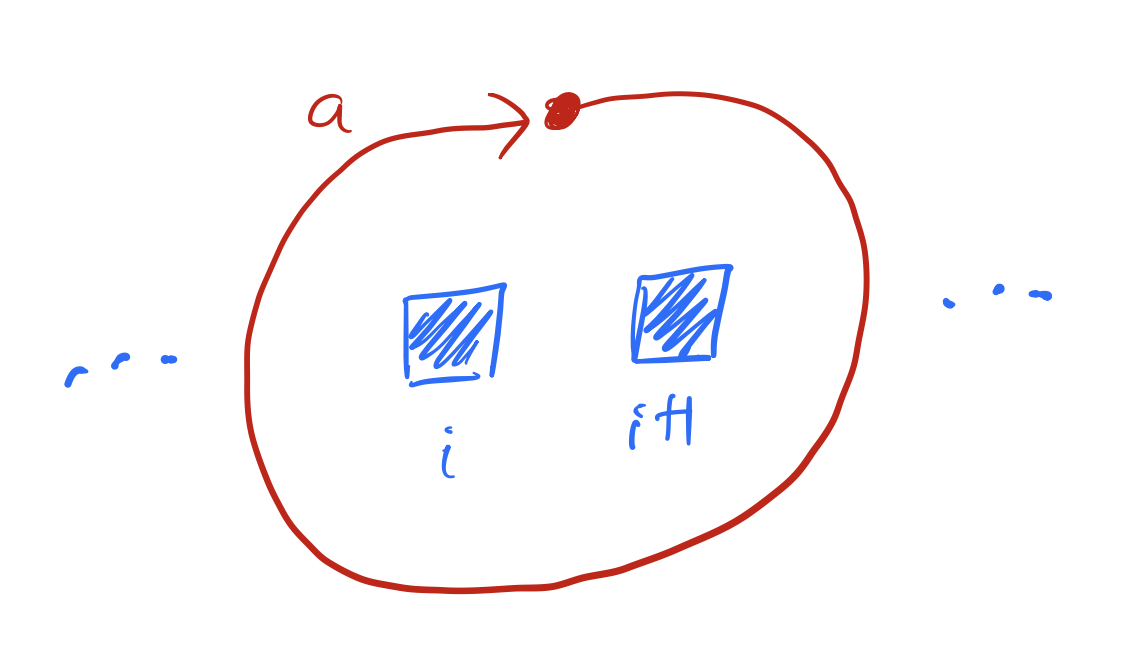
\includegraphics[scale=0.35]{Lectures/Images/lec10-anyonbraid.png}
\end{center}

Here, $a$ could be a flux or a charge. The other way to define trivial topological charge is whether the two fluxes can be created locally from the vacuum/ground state. But the former is a bit more operational, because it gives us a physical way to measure the topological charge (by measuring the Non-Abeliean Berry phase). This is the way in which we can distinguish degenerate ground states with each other.

We can now ask - what is the projection $P_{i,i+1}$ that projects onto the $i, i+1$st fluxes having trivial topological charge?

The answer (which we will then motivate the correctness of):
\begin{equation}\label{eq:projectionaction}
    \boxed{P_{i, i+1}\ket{\ldots, g_{i}, g_{i+1}, \ldots} = \delta_{g_ig_{i+1}, 1}\cdot\frac{1}{\abs{G}}\sum_h \ket{\ldots, hg_i h^{-1}, h g_{i+1}h^{-1}, \ldots}}
\end{equation}
Where we note that only $g_i, g_{i+1}$ get conjugated. Let us explain why we get the two factors.
\begin{enumerate}
    \item Why the $\delta_{g_ig_{i+1}, 1}$? This enforces $g_ig{i+1} = 1$,  which implies that $B_1(\gamma)\ket{\ldots, g_i, g_{i+1}, \ldots} = \ket{\ldots, g_i, g_{i+1}, \ldots}$ where $B_1(\gamma)$ is an operator that checks that the total flux is trivial inside of the loop (definition below, taking $C = 1$)
    \begin{center}
        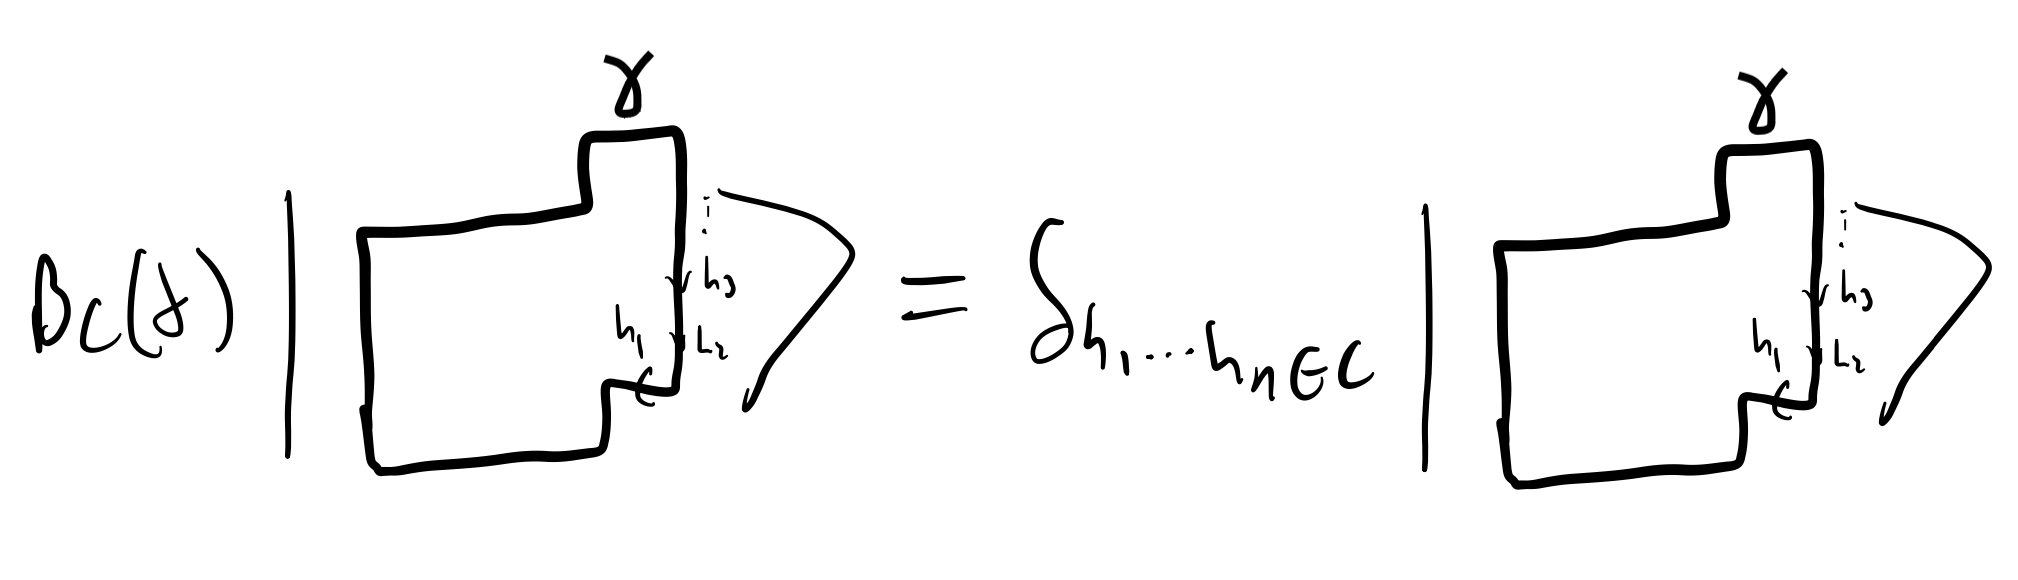
\includegraphics[scale=0.35]{Lectures/Images/lec8-Bcgamma.png}
    \end{center}
    This is a necessary condition to have trivial topological charge. It is 1 in the ground state, so if I am able to create the flux excitations locally, it also better be 1. It also has to do with the braiding of anyons, specifically charges; $B_1(\gamma) = 1$ implies we have trivial braiding with all charge excitations.
    \item Why a sum over conjugates of $g_i, g_{i+1}$? It comes from wanting to have trivial braiding with fluxes - we imagine braiding a flux $h$ around $g_{i}, g_{i+1}$. Assume that we have already fulfilled the $g_ig_{i+1} = 1$, so then $g_i = g_{i+1}^{-1} = g$.
    \begin{center}
        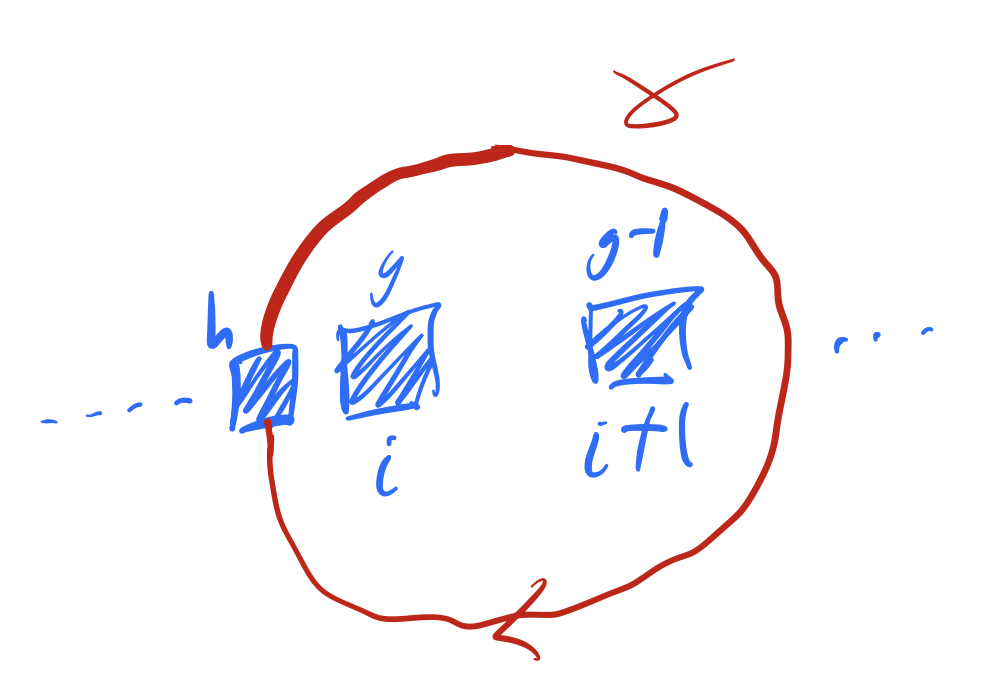
\includegraphics[scale=0.35]{Lectures/Images/lec10-mbraid.png}
    \end{center}

    It is then clear that we need the braiding process $\sigma_1\sigma_2\sigma_2\sigma_1$ to get the full braid of $h$ around the two fluxes:
    \begin{center}
        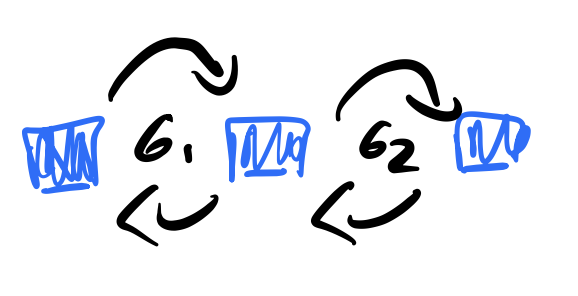
\includegraphics[scale=0.35]{Lectures/Images/lec10-sigmabraid.png}
    \end{center}

    Then it is only a matter of using Eq. \eqref{eq:fluxswaps} repeatedly:
    \begin{equation}
        \begin{split}
            \ket{\ldots, h, g, g^{-1}, \ldots} &\stackrel{\sigma_1}{\to} \ket{\ldots, hgh^{-1}, h, g^{-1}, \ldots}
            \\ &\stackrel{\sigma_2}{\to}\ket{\ldots, hgh^{-1}, hg^{-1}h^{-1}, h, \ldots}
            \\ &\stackrel{\sigma_2}{\to}\ket{\ldots, hgh^{-1}, hg^{-1}h^{-1}h(hg^{-1}h^{-1})^{-1}, hg^{-1}h^{-1}, \ldots} = \ket{\ldots, hgh^{-1}, hg^{-1}hgh^{-1}, hg^{-1}h^{-1}, \ldots}
            \\ &\stackrel{\sigma_1}{\to} \ket{\ldots, h, hgh^{-1}, hg^{-1}h^{-1}, \ldots}
        \end{split}
    \end{equation}
    So; if we braid $h$ around the two fluxes, nothing happens to the $h$ (makes sense as the total flux of the two is trivial) and the $g, g^{-1}$ fluxes get conjugated by $h$. The fact that we sum over all possible conjugates $\sum_h \ket{\ldots, hg_i h^{-1}, h g_{i+1}h^{-1}, \ldots}$ guarantees that braiding with fluxes will be a trivial operation.
\end{enumerate}
To summarize, there were two terms in the definition of our projection operation. The first term was there to have the braiding with charges to be trivial, the second term was there to have the braiding with fluxes to be trivial.